\chapter{Teoremas de la alternativa}
Los teoremas de la alternativa constituyen una potente herramienta en optimización. A pesar de tener un claro carácter convexo, se aplican incluso a problemas no convexos, tal y como se comprobará a lo largo de esta memoria. Nuestro punto de partida es el resultado del análisis  convexo, más importante, el teorema de Hahn-Banach. Es más, daremos una versión equivalente debida a H. König, conocida como el teorema de Mazur-Orlicz-König. Como consecuencia, obtendremos el teorema de la alternativa de Gordan, tanto en su versión convexa como una más general. 

\section{Teorema de Mazur-Orlicz-König}
El objetivo principal de esta sección es demostrar una versión equivalente no muy conocida del clásico teorema de Hanh-Banach, el teorema de Mazur-Orlicz-König. Iremos de una versión básica y algebraica del teorema de Hahn-Banach al teorema de Mazur-Orlicz-König siguiendo como aparece en el texto de S. Simons \cite{Simons2008}. \\
	
En primer lugar vamos a recordar la definición de funcional sublineal sobre un espacio vectorial \vecSpace . Notar que todos los espacios vectoriales que vamos a usar son reales. Del mismo modo, los espacios y conjuntos que usaremos asumiremos que son no vacíos.
	
\begin{definicion}
Sea \vecSpace un espacio vectorial. Decimos que el $P:\vecSpace \rightarrow \RR$ es sublineal si cumple las siguientes condiciones:
	\begin{itemize}
		\item $ P $ es subaditiva: $x_1, x_2 \in \vecSpace \Longrightarrow P(x_1 + x_2) \leq P(x_1) + P(x_2) $.
		\item $ P $ es positivamente homogénea: $x_1 \in \vecSpace $ y $ \lambda > 0 \Longrightarrow P(\lambda x) = \lambda P(x) $.
	\end{itemize}
\end{definicion}

Como consecuencia, podemos afirmar que $ P(0) = 0 $. En efecto:
\[
P(0) = P(2\times0) = 2\times P(0) \Longrightarrow P(0) = 0.
\]

Por ejemplo, toda norma o incluso toda seminorma sobre \vecSpace es un funcional sublineal. Así, dados $ a,b \in \RR $ con $ a <b $ tenemos que $ P:H^{1} (a,b) \longrightarrow \RR$ definida como \[ P(x) = \norm{x'}_{L^2(a,b)} \] es una seminorma y por ello sublineal. También, si $ \vecSpace = \RR $ y definimos la parte positiva \[ P(x) = [x]^{+} = \max \{0,x\}, \forall x \in \RR \] obtenemos un funcional sublineal sobre $\RR$. \\
	
El lema que exponemos a continuación, y que generalizaremos posteriormente en el lema \ref{lema2}, nos servirá para demostrar el teorema de Hanh-Banach. 
	
\bigskip
	\begin{lemaBox}\label{lema1}
		Sea\vecSpace un espacio vectorial y $P:\vecSpace \rightarrow \RR$ un funcional sublineal. Fijamos un elemento $ y \in \vecSpace $ y para todo $ x \in \vecSpace $ tomamos  
		\begin{center}
			$ P_y(x) := \displaystyle\inf_{\lambda > 0} \left[P(x+\lambda y) - \lambda P(y)\right] $
		\end{center}
		
		Entonces, $ P_y(\vecSpace) \subset \RR$, $ P_y:\vecSpace \longrightarrow \RR $ es sublineal, $ P_y \leq P $ y además $ P_y (-y) \leq  -P(y)$.
	\end{lemaBox} 
	\begin{proof}
		Fijamos $ y \in V $. Sea $ x \in V $ y $ \lambda > 0$. Como P es sublineal tenemos: 
		\begin{center}
			$ \lambda P(y) = P(\lambda y) =P(\lambda y +x-x) \leq P(x+\lambda y)+ P(-x)$.
		\end{center}
		Por lo tanto, se obtiene que $ P(x+\lambda y) - \lambda P(y) \geq -P(-x) $.  Tomando el ínfimo sobre $ \lambda >0 $ llegamos a $ P_{y}(x)\geq -P(-x) > -\infty$. Por consiguiente, $ P_y(\vecSpace) \subset \RR$, esto es $ P_y:\vecSpace \longrightarrow \RR $. \\
		
		Probaremos ahora que $ P_y $ es sublineal. Empezamos viendo la subaditividad. Tomamos $ x_1, x_2 \in V $ y sean $ \lambda_1, \lambda_2 > 0$ arbitrarios. Entonces, la definición de $ P_y $ da 
		\begin{equation*}
		\begin{split}
		( P(x_1 + \lambda_1 y) - \lambda_1 P(y) ) &+ ( P(x_2 + \lambda_2 y) - \lambda_2 P(y) ) \\
		& \geq ( P(x_1 + x_2 + (\lambda_1+\lambda_2)y)) - (\lambda_1+\lambda_2) P(y) \\
		&\geq P_y (x_1 + x_2 ).
		\end{split}
		\end{equation*}
		Tomando ínfimos sobre $ \lambda_1 $ y $ \lambda_2 $, $  P_y (x_1)  + P_y (x_2 ) \geq P_y (x_1 + x_2 ) $. Así, $ P_y $ es subaditiva. Para comprobar que es positivamente homogénea tomamos $ x \in V $ y $ \mu > 0 $. Entonces:
		\begin{equation*}
		\begin{split}
		P_y (\mu x) &= \inf_{\lambda > 0} \left[P(\mu x+\lambda y) - \lambda P(y)\right] \\
		&= \mu \inf_{\lambda > 0} \left[P(x+ (\lambda / \mu) y) - (\lambda / \mu) P(y)\right] \\
		&= \mu \inf_{\upsilon > 0} \left[P(x+ \upsilon y) - \upsilon  P(y)\right] \\
		&= \mu P_y (x).
		\end{split}
		\end{equation*}	
		Obtenemos que $ P_y $ es positivamente homogénea y como consecuencia sublineal. \\
		
		Para demostrar que $ P_y \leq P $, sea $ x \in V $ y tomando $ \lambda = 1 $ en la definición de $ P_y $,
		\[ P_y(x) \leq P(x+y) - P(y) \leq P(x)+ P(y) - P(y) = P(x) \]
		Como $ x \in \vecSpace $ es arbitrario, entonces $ P_y \leq P $. Finalmente, razonando de manera similar,
		\[P_y(-y) \leq P(-y+y) - P(y) = -P(y).  \]
		
	\end{proof}
\bigskip
El teorema de Hahn-Banach que hemos mencionado antes (básico y algebraico) se enuncia en estos términos:

\bigskip
	\begin{teoremaBox}[Hanh-Banach]\label{H-B}
		Sea V un espacio vectorial y $P:V \rightarrow \RR$ un funcional sublineal. Entonces existe un funcional lineal $ L:\vecSpace \longrightarrow \RR $ tal que $ L \leq P $.
	\end{teoremaBox}
\begin{figure}[h!]
	%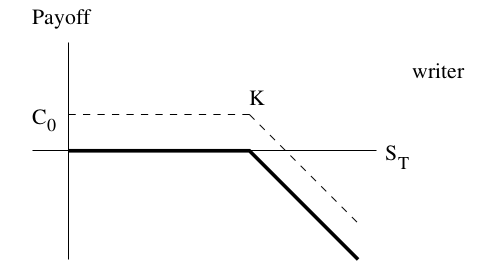
\includegraphics[width=1\linewidth]{Writer_call}
	\centering
	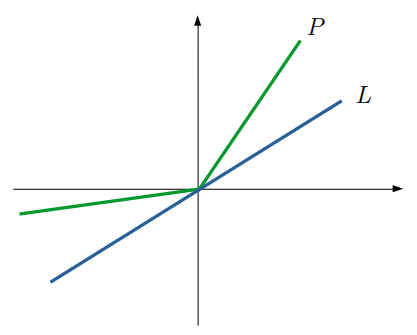
\includegraphics[width=0.6\linewidth]{H-B}
	\caption{Teorema de Hahn-Banach.}
\end{figure}

	\begin{proof}
		Sea $ \text{SUB} = \lbrace Q:\vecSpace \longrightarrow \RR : Q \leq P \rbrace$, es decir, el conjunto de funcionales sublineales sobre \vecSpace que minoren a $ P $. Nuestro propósito es emplear el lema de Zorn con objeto de probar que tiene un elemento minial y tal elemento será el funcional $ L $ que buscamos. Para ello, dados $ T_1 ,T_2 \in \text{SUB} $ consideramos la relación de orden usual, es decir:
		\begin{center}
			$ T_1 \leq T_2 \Longleftrightarrow T_1 (x) \leq T_2 (x) \quad \forall x \in \vecSpace $.
		\end{center}
		Primero probaremos que todo subconjunto $ \mathcal{T} $ totalmente ordenado de $SUB $ tiene una cota inferior en  SUB. Definimos $ Q(x):=\inf \{ T(x): T \in \mathcal{T} \} $ y queremos ver que $ Q(x) \in \RR $. Si $ x \in \vecSpace $ y $ T \in \mathcal{T} $, como T es subaditiva obtenemos la siguiente relación:
		\[ 0 = T(0) = T(x-x) \leq T(x) + T(-x) \Longrightarrow T(x) \geq -T(-x) \quad (1)\]  
		Por otro lado:
		\[ T \in \mathcal{Q} \Longrightarrow T(x) \leq P(x) \Longrightarrow -T(x) \geq -P(x) \quad (2)\] 
		Usando (1), (2) y tomando ínfimo sobre $  T $  llegamos a $ Q(x) \geq -P(x) \geq - \infty $. Por lo tanto $ Q:V \rightarrow \RR$. \\
		
		Ahora probaremos que $ Q $ es subaditiva. Para ello, tomamos $ x_1, x_2\in \vecSpace $. Sean $ T_1 , T_2 \in \mathcal{T} $ arbitrarios. Si $ T_1 \geq T_2 $ (el caso de $ T_2 \geq T_1 $ es análogo.):
		
		\begin{center}
			$ T_1 (x_1)+  T_2 (x_2) \geq T_2(x_1)+  T_2 (x_2) \geq T_2(x_1 +x_2) \geq Q(x_1 + x_2).$
		\end{center}
		Concluimos (en ambos casos) que $ T_1 (x_1)+  T_2 (x_2) \geq Q(x_1 + x_2)$. Tomando ínfimo en $ T_1 $ y $ T_2 $ obtenemos que $ Q (x_1)+  Q(x_2) \geq Q(x_1 + x_2)$. Así, $ Q $ es sublineal. Que sea positivamente homogénea es consecuencia de que $ T $ también lo es. Dado $ \mu > 0 $:
		\begin{equation*}
		\begin{split}
		Q(\mu x) &=\inf \{ T(\mu x): T \in \mathcal{T} \} \\ 
		& = \inf \{ \mu T( x): T \in \mathcal{T} \} \\ 
		&= \mu\inf \{ T( x): T \in \mathcal{T} \} \\ 
		&= \mu Q(x). 
		\end{split}
		\end{equation*}
		
		De este modo, Q es sublineal y como es claro que $ Q \leq P \Longrightarrow Q \in \text{SUB} $. Así, es directo que $ Q $ es el elemento minimal de $ \mathcal{T} $ en SUB.\\
		
		El lema de Zorn nos proporciona entonces un elemento minimal de SUB que llamaremos $ L $. Vamos a comprobar que $ L $ es lineal y, por tanto, es el funcional buscado. Tomamos ahora $ y \in \vecSpace $. Con la notación del lema anterior, $ L_y : \vecSpace \longrightarrow \RR $ es sublineal, $ L_y \leq L $ (como consecuencia $ L_y \in \text{SUB} $) y $ L_y (-y) \leq L(-y) $. De hecho, como $ L $ es minimal en SUB, $ L_y = L $ y por ello $ L (-y) \leq L(-y) $. Por otro lado, como L es subaditiva, $ L(-y) \geq -L(y) $. Combinando ambas desigualdades, $ L(-y) = -L(y) $. Tomamos $ x \in \vecSpace $ y $ \lambda < 0 $, usando la igualdad anterior llegamos a:
		\[ \qquad \quad
		L(\lambda x) = L (-(-\lambda)x) = -L(-\lambda x) = -(-\lambda)L(x) = \lambda L(x) \label{1}
		\] 
		obteniendo que $ L $ es homogénea. Si $ x_1, x_2 \in \vecSpace $, la subaditividad de $ L $ nos da $ L(-x_1-x_2) \leq L(-x_1) + L(-x_2) $. Usando la homogeneidad de $ L $:
		\begin{equation*}
		\begin{split} \qquad
		L(x_1+x_2) &= L(-(-x_1-x_2)) = -L(-x_1-x_2) \\ 
		& \geq -L(-x_1)-L(-x_2) = L(x_1) + L (x_2) \geq L(x_1+x_2). 
		\end{split}
		\end{equation*}
		Por ello, $	L(x_1+x_2) = L(x_1) + L (x_2) $ y por la arbitrariedad de $ x_1, x_2 \in \vecSpace $ concluimos que $ L $ es lineal.
		
	\end{proof}
\bigskip

Nos disponemos a probar, a partir de el teorema de Hahn-Banach el de Mzur-Orlicz-König, que supone un refinamiento. Antes, necesitamos un resultado técnico, que constituye una especie de versión global sobre un convexo del lema \ref{lema1}.
	
\bigskip 
	\begin{lemaBox}\label{lema2}
		Sea\vecSpace un espacio vectorial y $P:\vecSpace \rightarrow \RR$ un funcional sublineal. Sea $ D $ un subconjunto convexo de \vecSpace y sea $ \beta := \inf_D P \in \RR $. Para todo $ x \in V $ tomamos  
		\begin{center}
			$ Q(x) := \inf_{d \in D, \lambda > 0} \left[P(x+\lambda d) - \lambda \beta\right] $
		\end{center}
		
		Entonces, $ Q(\vecSpace) \subset \RR $, $ Q:V \rightarrow \RR$ es sublineal, $ Q \leq P $ y además $ \forall d \in D$ se cumple  $-Q(-d) \geq \beta$.
	\end{lemaBox} 
	\begin{proof}
		Si $ x \in \vecSpace,\text{ }d \in D $ y $ \lambda > 0 $, entonces
		\begin{center}
			$ P(x+ \lambda d) - \lambda \beta \geq -P(-x) + \lambda P(d)-\lambda\beta \geq -P(-x) \geq -\infty$.
		\end{center}
		La primera desigualdad se deduce de la linealidad de P ya que:
		\begin{equation*}
		\begin{split}
		\lambda P(d) &= P(\lambda d) \\ 
		&=P(\lambda d +x-x) \\ 
		&\leq P(x+\lambda d)+ P(-x)
		\end{split}
		\end{equation*}
		por lo que $ \lambda P(d)-P(-x) \leq P(x+\lambda d) $. La segunda se debe a que
		\[\beta = \inf_D P \Longrightarrow \lambda P(d) \geq \lambda\beta \Longrightarrow\lambda P(d) - \lambda\beta \geq 0. \]
		Tomando el ínfimo sobre $ d \in D  $ y $ \lambda > 0 $ llegamos a \[ Q(x)\geq -P(-x) > -\infty,\] por lo que $ Q(\vecSpace) \longrightarrow \RR$. Es relativamente fácil probar que $ Q $ es positivamente homogénea por lo que para ver que es sublineal solo queda comprobar la subaditividad. Para ello, tomamos $ x_1, x_2 \in V $. Sean $ d_1, d_2 \in D $ y $ \lambda_1, \lambda_2 > 0$ arbitrarios. Para simplificar la notación llamamos $ x := x_1 + x_2 $, $ \lambda := \lambda_1 + \lambda_2 $ y $ d:= (\lambda_1/\lambda)d_1 + (\lambda_2/\lambda)d_2 $. Notar que $ d \in D $, al ser este convexo. Entonces: 
		\begin{equation*}
		\begin{split}
		( P(x_1 + \lambda_1 d_1) - \lambda_1 \beta ) + ( P(x_2 + \lambda_2 d_2) - \lambda_2 \beta ) &\geq P(x + \lambda_1 d_1 + \lambda_2 d_2) - \lambda \beta\\
		& = P(x +\lambda d) - \lambda \beta\\ 
		& \geq Q(x) = Q(x_1 + x_2).
		\end{split}
		\end{equation*}
		Tomando ínfimo sobre $ d_1, d_2, \lambda_1 $ y $ \lambda_2 $, $  Q(x_1) + Q (x_2 ) \geq Q (x_1 + x_2 ) $. Así, $ Q $ es subaditiva y como consecuencia sublineal. Para concluir, fijamos $ d \in D $. Sea $ x \in \vecSpace $ arbitrario. Entonces, $ \forall \lambda > 0 $, $ Q(x) \leq P(x) + \lambda (P(d) - \beta )$. Tomando $ \lambda \longrightarrow 0 $, $ Q(x) \leq P(x)$ y como consecuencia $ Q \leq P $. Finalmente, sea $ d \in D $ arbitrario y tomando $ \lambda = 1 $:
		\[Q(-d) \leq Q(-d+d) - \beta = -\beta \Longrightarrow  -Q(-d) \geq \beta.  \]
		
	\end{proof}
\bigskip

Ya estamos preparados para probar el teorema de Mazur-Orlicz-König, debido a H. König \cite{König1, König2}. No solo es una versión equivalente del teorema de Hahn-Banach, también de un teorema de Mazur-Orlicz \cite{mo}, aunque es solo una reformulación. 

\bigskip
	
	\begin{teoremaBox}[Mazur-Orlicz-König]\label{M-O}
		Sea\vecSpace un espacio vectorial y $P:\vecSpace \rightarrow \RR$ un funcional sublineal.  Sea $ D $ un subconjunto no vacío y convexo de \vecSpace. Entonces existe un funcional $ L: \vecSpace \longrightarrow \RR $ lineal tal que $ L \leq P $ e $ \inf_D L = \inf_D P $.
	\end{teoremaBox}

Antes de pasar a la demostración, observemos que, aunque es un resultado puramente algebraico, tiene una fuerte interpretación geométrica: el teorema de Hahn-Banach garantiza, dado un funcional sublineal, $ P: \vecSpace \longrightarrow \RR $, la existencia de un funcional lineal $ L:\vecSpace \longrightarrow \RR $ con $ L \leq P $. En la imagen \ref{H-B-varios} mostramos unos ejemplos de funcionales que nos aporta el teorema de Hahn-Banach. \\

\begin{figure}[h!]
	%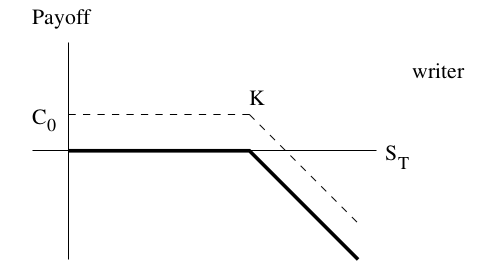
\includegraphics[width=1\linewidth]{Writer_call}
	\centering
	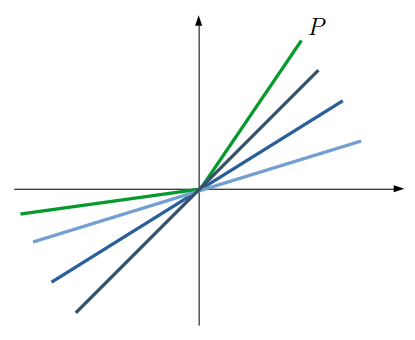
\includegraphics[width=0.6\linewidth]{H-B_2}
	\caption{Ejemplos de funcionales aportados por el teorema de Hahn-Banach.}
	\label{H-B-varios}
\end{figure} 

El teorema de Mazir-Orlicz-König, fijado un subconjunto convexo $ D $ de $ \vecSpace $, nos da solo los funcionales lineales que minoran a $ P $ y que cumplen
\[
\inf_D L = \inf_D P.
\]
En la imagen \ref{M-O-K-fotos} se muestra un ejemplo del teorema.
\begin{figure}[h!]
	%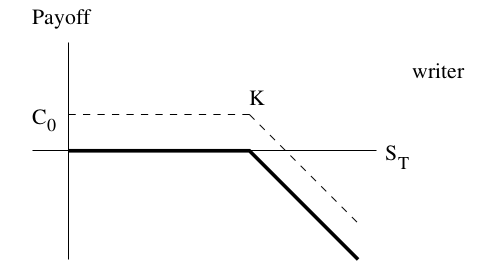
\includegraphics[width=1\linewidth]{Writer_call}
	\centering
	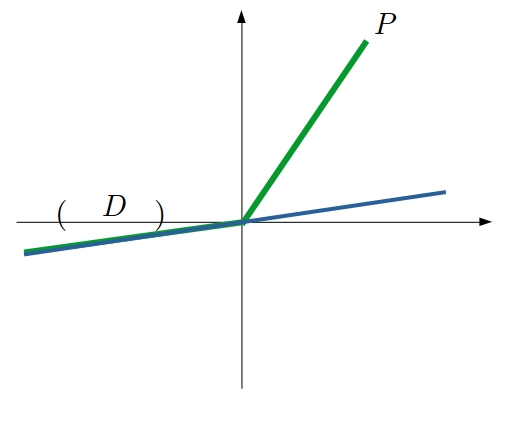
\includegraphics[width=0.6\linewidth]{M-O-K}
	\caption{Teorema de Mazur-Orlicz-König.}
	\label{M-O-K-fotos}
\end{figure} 

	\begin{proof}
		Sea $ \beta := \inf_D P $. En el caso de que $ \beta = -\infty $ por el teorema de Hanh-Banach tenemos que $ \exists L $ sobre \vecSpace tal que es lineal y $ L \leq P$. Así:
		\begin{center}
			$ L \leq P \Longrightarrow inf_D L \leq \inf_D P = -\infty \Longrightarrow inf_D L = \inf_D P.$ 
		\end{center}
		Supongamos entonces que $ \beta \in \RR $. Definimos el funcional auxiliar $ Q $ como en el lema \ref{lema2}. Del teorema de Hanh-Banach obtenemos que existe un funcional lineal $ L $ sobre \vecSpace tal que $ L \leq Q$ (como $ Q \leq P $ tenemos que $ L \leq P $). Sea $ d \in D $, entonces:
		\[
		L(d) = -L(-d) \geq -Q(-d) \geq \beta.
		\]
		Tomando ínfimo sobre $ d \in D $:
		\[
		\inf_D L \geq \beta = \inf_D P.
		\]
		Por otro lado, como $ L \geq P $:
		\[
		\inf_D L \leq\inf_D P.
		\]
		Juntando ambas desigualdades obtenemos $ \inf_D L =\inf_D P $.
	\end{proof}

\bigskip
